\section{Overview}

We provide an overview of the code transformation software.
The software input is a single-GPU-based ML model code package
that include a training code.
The software parses the Python code files in the package
into AST format, apply an appropriate transformation on the AST,
and generates an output code package that corresponds to
the distributed training code.

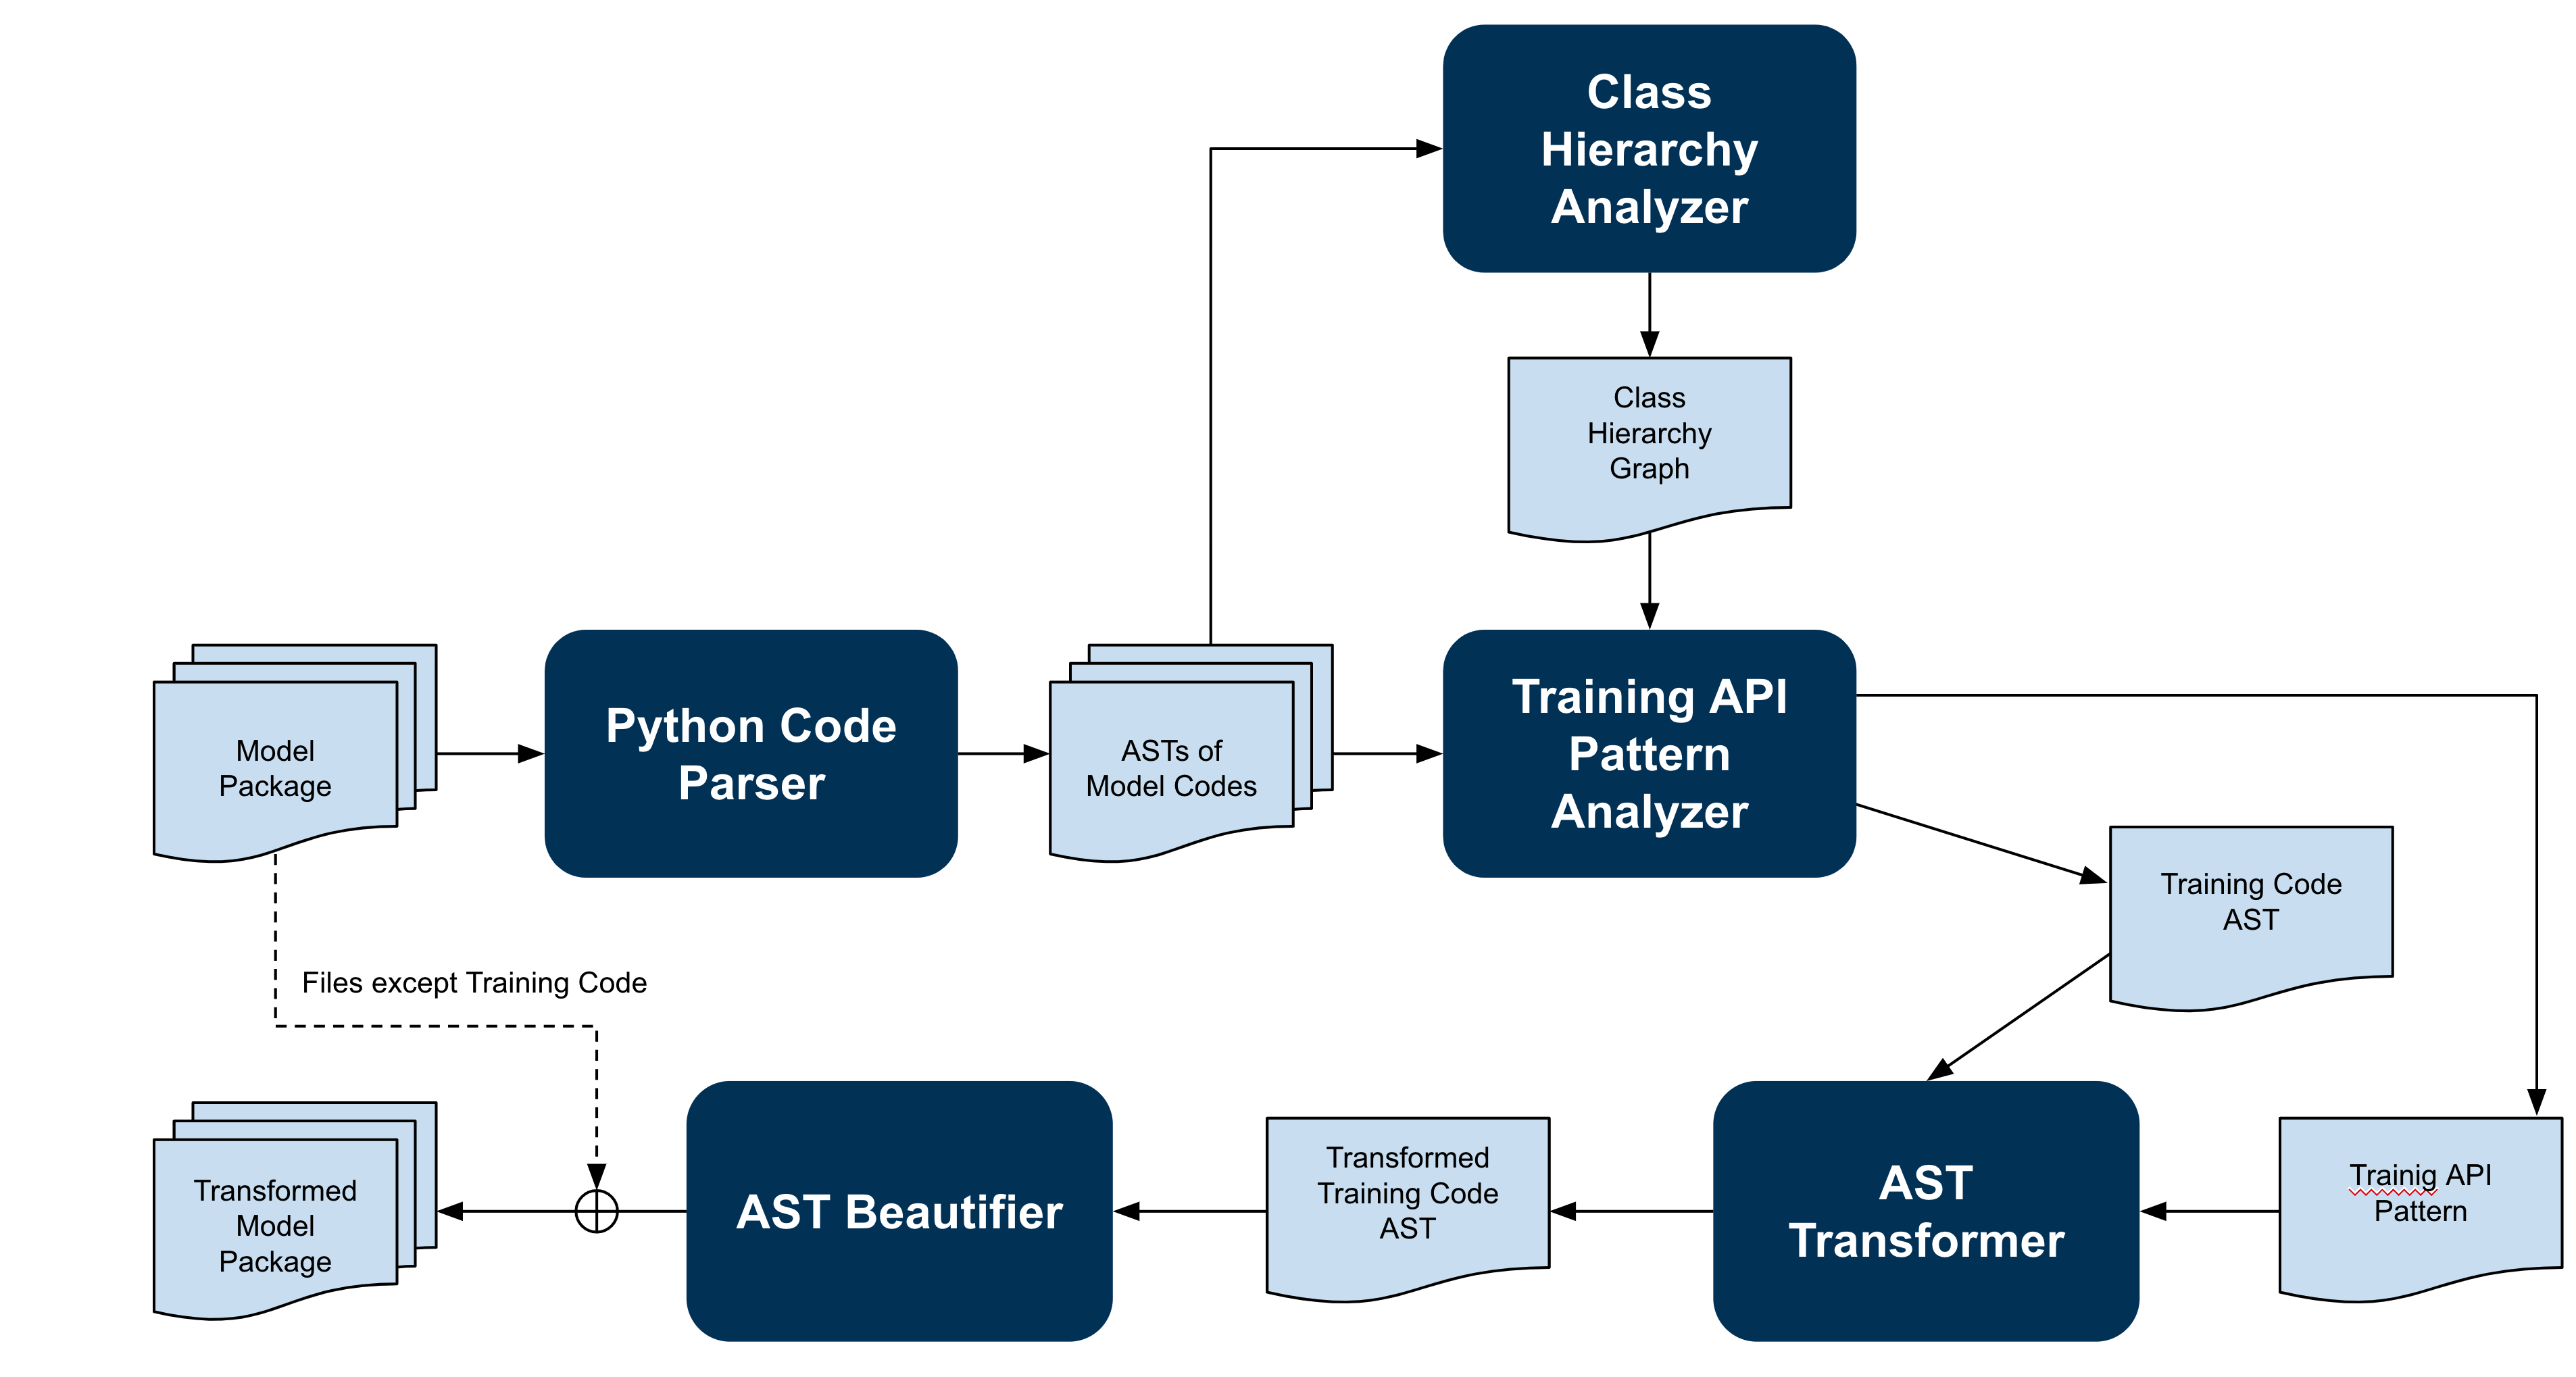
\includegraphics[width=1\textwidth]{system_arch}

The system is composed of five modules: the input parser,
the class hierarchy analyzer, the API pattern analyzer,
the AST transformer, and the output code generator.

\subsection{Parser}

The parser module is responsible of locating Python code files in the
input ML model package and parsing each into corresponding AST.
We refer to the Python lanugage reference\cite{pythonref}
to define Python abstract syntax and Python parser.
The Python abstract syntax and the parser 
are described in the Section \ref{sec:trans}.

\subsection{Class Hierarchy Analyzer}


\vspace{-3em}
\begin{figure}[h]
  \lstinputlisting[language=Python]{motiv_ex.py}
\end{figure}
\vspace{-3em}

To correctly transform TensorFlow training codes,
the transformation software requires subclassing relationship
between user-defined classes and TensorFlow library classes.
In the above code example, for instance, the software need to recognize
the {\tt model.fit} method call as an training API.
To recognize this, the software should identify the user-defined class
{\tt ResNet} as a subclass of the TensorFlow class {\tt keras.models.Model},
so that the {\tt ResNet} instance {\tt model} inherits the {\tt fit}
method from the parent class. 
We implemented the class hierarchy analyzer for Python code package
to generate the class hierarchy graph which is utilized by
other modules. The details of the class hierarchy analyzer is
described in the Section \ref{sec:cha}.

\subsection{Training API Pattern Analyzer}

Training API pattern analyzer is responsible of identifying
TensorFlow training APIs occur in the input code and select appropriate
transformation rule.

\subsection{AST Transformer}

The AST transformer module transforms the input AST into the output AST.
